\PassOptionsToPackage{unicode=true}{hyperref} % options for packages loaded elsewhere
\PassOptionsToPackage{hyphens}{url}
%
\documentclass[]{article}
\usepackage{lmodern}
\usepackage{amssymb,amsmath}
\usepackage{ifxetex,ifluatex}
\usepackage{fixltx2e} % provides \textsubscript
\ifnum 0\ifxetex 1\fi\ifluatex 1\fi=0 % if pdftex
  \usepackage[T1]{fontenc}
  \usepackage[utf8]{inputenc}
  \usepackage{textcomp} % provides euro and other symbols
\else % if luatex or xelatex
  \usepackage{unicode-math}
  \defaultfontfeatures{Ligatures=TeX,Scale=MatchLowercase}
\fi
% use upquote if available, for straight quotes in verbatim environments
\IfFileExists{upquote.sty}{\usepackage{upquote}}{}
% use microtype if available
\IfFileExists{microtype.sty}{%
\usepackage[]{microtype}
\UseMicrotypeSet[protrusion]{basicmath} % disable protrusion for tt fonts
}{}
\IfFileExists{parskip.sty}{%
\usepackage{parskip}
}{% else
\setlength{\parindent}{0pt}
\setlength{\parskip}{6pt plus 2pt minus 1pt}
}
\usepackage{hyperref}
\hypersetup{
            pdftitle={Who am I},
            pdfauthor={Haoxi Ma},
            pdfborder={0 0 0},
            breaklinks=true}
\urlstyle{same}  % don't use monospace font for urls
\usepackage[margin=1in]{geometry}
\usepackage{color}
\usepackage{fancyvrb}
\newcommand{\VerbBar}{|}
\newcommand{\VERB}{\Verb[commandchars=\\\{\}]}
\DefineVerbatimEnvironment{Highlighting}{Verbatim}{commandchars=\\\{\}}
% Add ',fontsize=\small' for more characters per line
\usepackage{framed}
\definecolor{shadecolor}{RGB}{248,248,248}
\newenvironment{Shaded}{\begin{snugshade}}{\end{snugshade}}
\newcommand{\AlertTok}[1]{\textcolor[rgb]{0.94,0.16,0.16}{#1}}
\newcommand{\AnnotationTok}[1]{\textcolor[rgb]{0.56,0.35,0.01}{\textbf{\textit{#1}}}}
\newcommand{\AttributeTok}[1]{\textcolor[rgb]{0.77,0.63,0.00}{#1}}
\newcommand{\BaseNTok}[1]{\textcolor[rgb]{0.00,0.00,0.81}{#1}}
\newcommand{\BuiltInTok}[1]{#1}
\newcommand{\CharTok}[1]{\textcolor[rgb]{0.31,0.60,0.02}{#1}}
\newcommand{\CommentTok}[1]{\textcolor[rgb]{0.56,0.35,0.01}{\textit{#1}}}
\newcommand{\CommentVarTok}[1]{\textcolor[rgb]{0.56,0.35,0.01}{\textbf{\textit{#1}}}}
\newcommand{\ConstantTok}[1]{\textcolor[rgb]{0.00,0.00,0.00}{#1}}
\newcommand{\ControlFlowTok}[1]{\textcolor[rgb]{0.13,0.29,0.53}{\textbf{#1}}}
\newcommand{\DataTypeTok}[1]{\textcolor[rgb]{0.13,0.29,0.53}{#1}}
\newcommand{\DecValTok}[1]{\textcolor[rgb]{0.00,0.00,0.81}{#1}}
\newcommand{\DocumentationTok}[1]{\textcolor[rgb]{0.56,0.35,0.01}{\textbf{\textit{#1}}}}
\newcommand{\ErrorTok}[1]{\textcolor[rgb]{0.64,0.00,0.00}{\textbf{#1}}}
\newcommand{\ExtensionTok}[1]{#1}
\newcommand{\FloatTok}[1]{\textcolor[rgb]{0.00,0.00,0.81}{#1}}
\newcommand{\FunctionTok}[1]{\textcolor[rgb]{0.00,0.00,0.00}{#1}}
\newcommand{\ImportTok}[1]{#1}
\newcommand{\InformationTok}[1]{\textcolor[rgb]{0.56,0.35,0.01}{\textbf{\textit{#1}}}}
\newcommand{\KeywordTok}[1]{\textcolor[rgb]{0.13,0.29,0.53}{\textbf{#1}}}
\newcommand{\NormalTok}[1]{#1}
\newcommand{\OperatorTok}[1]{\textcolor[rgb]{0.81,0.36,0.00}{\textbf{#1}}}
\newcommand{\OtherTok}[1]{\textcolor[rgb]{0.56,0.35,0.01}{#1}}
\newcommand{\PreprocessorTok}[1]{\textcolor[rgb]{0.56,0.35,0.01}{\textit{#1}}}
\newcommand{\RegionMarkerTok}[1]{#1}
\newcommand{\SpecialCharTok}[1]{\textcolor[rgb]{0.00,0.00,0.00}{#1}}
\newcommand{\SpecialStringTok}[1]{\textcolor[rgb]{0.31,0.60,0.02}{#1}}
\newcommand{\StringTok}[1]{\textcolor[rgb]{0.31,0.60,0.02}{#1}}
\newcommand{\VariableTok}[1]{\textcolor[rgb]{0.00,0.00,0.00}{#1}}
\newcommand{\VerbatimStringTok}[1]{\textcolor[rgb]{0.31,0.60,0.02}{#1}}
\newcommand{\WarningTok}[1]{\textcolor[rgb]{0.56,0.35,0.01}{\textbf{\textit{#1}}}}
\usepackage{graphicx,grffile}
\makeatletter
\def\maxwidth{\ifdim\Gin@nat@width>\linewidth\linewidth\else\Gin@nat@width\fi}
\def\maxheight{\ifdim\Gin@nat@height>\textheight\textheight\else\Gin@nat@height\fi}
\makeatother
% Scale images if necessary, so that they will not overflow the page
% margins by default, and it is still possible to overwrite the defaults
% using explicit options in \includegraphics[width, height, ...]{}
\setkeys{Gin}{width=\maxwidth,height=\maxheight,keepaspectratio}
\setlength{\emergencystretch}{3em}  % prevent overfull lines
\providecommand{\tightlist}{%
  \setlength{\itemsep}{0pt}\setlength{\parskip}{0pt}}
\setcounter{secnumdepth}{0}
% Redefines (sub)paragraphs to behave more like sections
\ifx\paragraph\undefined\else
\let\oldparagraph\paragraph
\renewcommand{\paragraph}[1]{\oldparagraph{#1}\mbox{}}
\fi
\ifx\subparagraph\undefined\else
\let\oldsubparagraph\subparagraph
\renewcommand{\subparagraph}[1]{\oldsubparagraph{#1}\mbox{}}
\fi

% set default figure placement to htbp
\makeatletter
\def\fps@figure{htbp}
\makeatother


\title{Who am I}
\author{Haoxi Ma}
\date{2019-02-28}

\begin{document}
\maketitle

\textbf{\emph{``I hope no longer feel guilty for life, every time I
memorise''}}

I am Haoxi Ma, hard-working and enterprising. Like most of you, I have
several real friends and a harmonious family. Life to me isn't very
tough but still with some pity.

If you want to know more\ldots{}

\textbf{· Grow from failure:}

\begin{Shaded}
\begin{Highlighting}[]
\KeywordTok{library}\NormalTok{(ggplot2)}
\end{Highlighting}
\end{Shaded}

\begin{verbatim}
## Warning: package 'ggplot2' was built under R version 3.6.2
\end{verbatim}

\begin{Shaded}
\begin{Highlighting}[]
\NormalTok{Time<-}\KeywordTok{c}\NormalTok{(}\StringTok{"2012Fall"}\NormalTok{,}\StringTok{"2013Spring"}\NormalTok{,}\StringTok{"2013Fall"}\NormalTok{,}\StringTok{"2014Spring"}\NormalTok{,}\StringTok{"2014Fall"}\NormalTok{,}\StringTok{"2015Spring"}\NormalTok{,}\StringTok{"2015Fall"}\NormalTok{,}\StringTok{"2016Spring"}\NormalTok{,}\StringTok{"2016Fall"}\NormalTok{,}\StringTok{"2017Spring"}\NormalTok{,}\StringTok{"2017Fall"}\NormalTok{,}\StringTok{"2018Spring"}\NormalTok{,}\StringTok{"2018Fall"}\NormalTok{,}\StringTok{"2019Spring"}\NormalTok{,}\StringTok{"2019Fall"}\NormalTok{,}\StringTok{"2020Spring"}\NormalTok{,}\StringTok{"2020Fall"}\NormalTok{)}
\NormalTok{GPA<-}\KeywordTok{c}\NormalTok{(}\FloatTok{3.8}\NormalTok{,}\FloatTok{3.9}\NormalTok{,}\FloatTok{3.95}\NormalTok{,}\FloatTok{3.9}\NormalTok{,}\FloatTok{4.0}\NormalTok{,}\FloatTok{4.0}\NormalTok{,}\FloatTok{3.2}\NormalTok{,}\FloatTok{3.0}\NormalTok{,}\FloatTok{2.5}\NormalTok{,}\FloatTok{2.4}\NormalTok{,}\FloatTok{3.8}\NormalTok{,}\FloatTok{4.0}\NormalTok{,}\FloatTok{3.9}\NormalTok{,}\FloatTok{4.0}\NormalTok{,}\FloatTok{4.0}\NormalTok{,}\FloatTok{4.0}\NormalTok{,}\FloatTok{4.0}\NormalTok{)}
\NormalTok{GPA.plot<-}\KeywordTok{data.frame}\NormalTok{(Time,GPA)}
\NormalTok{GPA.plot}\OperatorTok{$}\NormalTok{Time<-}\KeywordTok{factor}\NormalTok{(GPA.plot}\OperatorTok{$}\NormalTok{Time,}\DataTypeTok{levels =}\NormalTok{ Time)}
\NormalTok{gg_GPA<-}\KeywordTok{ggplot}\NormalTok{(GPA.plot,}\KeywordTok{aes}\NormalTok{(}\DataTypeTok{x=}\NormalTok{Time,}\DataTypeTok{y=}\NormalTok{GPA,}\DataTypeTok{group=}\DecValTok{1}\NormalTok{))}\OperatorTok{+}\KeywordTok{geom_line}\NormalTok{(}\DataTypeTok{col=}\StringTok{"dark blue"}\NormalTok{,}\DataTypeTok{size=}\FloatTok{1.5}\NormalTok{)}\OperatorTok{+}
\StringTok{  }\KeywordTok{geom_point}\NormalTok{(}\DataTypeTok{size=}\DecValTok{3}\NormalTok{,}\DataTypeTok{col=}\StringTok{"dark blue"}\NormalTok{)}\OperatorTok{+}\KeywordTok{ylim}\NormalTok{(}\DecValTok{0}\NormalTok{,}\DecValTok{4}\NormalTok{)}\OperatorTok{+}\KeywordTok{scale_x_discrete}\NormalTok{(}\DataTypeTok{breaks =} \KeywordTok{levels}\NormalTok{(GPA.plot}\OperatorTok{$}\NormalTok{Time)[}\KeywordTok{c}\NormalTok{(T, }\KeywordTok{rep}\NormalTok{(F, }\DecValTok{1}\NormalTok{))])}\OperatorTok{+}
\StringTok{    }\KeywordTok{labs}\NormalTok{(}\DataTypeTok{title=}\StringTok{"GPA from High school to Graduate"}\NormalTok{,}\DataTypeTok{subtitle=}\StringTok{"Shown by semester"}\NormalTok{,}\DataTypeTok{x=}\StringTok{"Semester"}\NormalTok{,}\DataTypeTok{y=}\StringTok{"GPA"}\NormalTok{)}\OperatorTok{+}
\StringTok{  }\KeywordTok{theme}\NormalTok{()}
  
\KeywordTok{plot}\NormalTok{(gg_GPA)}
\end{Highlighting}
\end{Shaded}

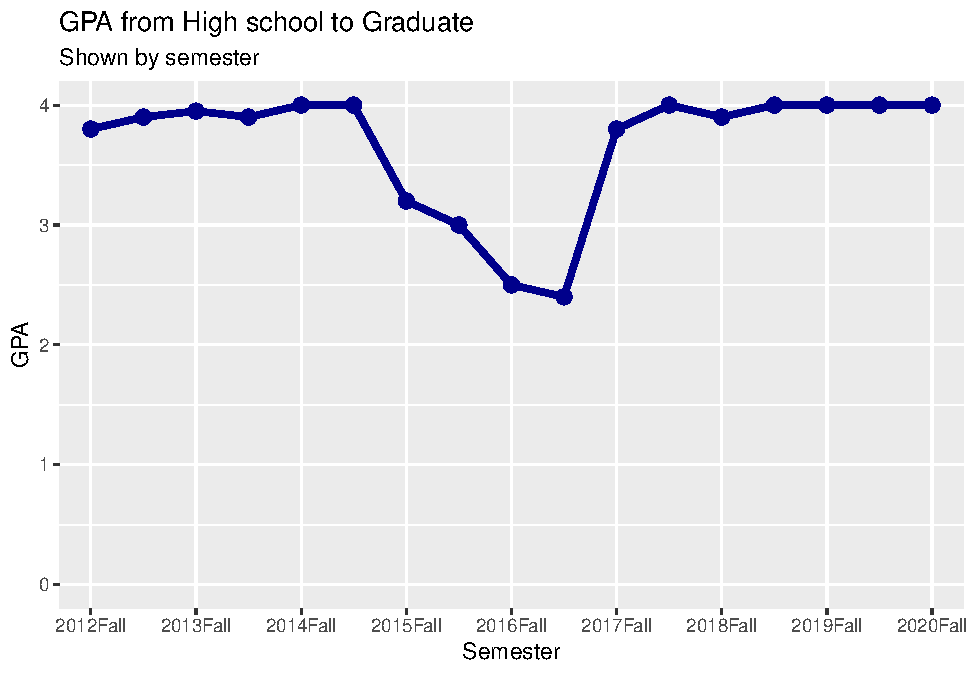
\includegraphics{about_files/figure-latex/unnamed-chunk-1-1.pdf}

\end{document}
